\apendice{Documentación de usuario}

\section{Introducción}

En esta sección explicaremos lo necesario para que los usuarios puedan instalar y utilizar la aplicación.

\section{Requisitos de usuarios}

El usuario, para poder utilizar la aplicación, deberá tener instalado \textit{Python}, al menos la versión 3.6.8 y cargar el entorno virtual que se ha creado con la ayuda del archivo \texttt{environment.yml}. Idealmente, el sistema se instalará en Windows 10, ya que la aplicación está optimizada para este sistema operativo.

\section{Instalación}

Los pasos para la instalación del proyecto se detallan en \nameref{instalacion}. Les resumimos:

\begin{itemize}
    \item Primero compruebe que ha descargado todos los archivos como indica el apartado \label{descargar}.
    \item Cree el entorno virtual y actívelo.
    \item Compruebe que las bibliotecas de OpenCV y TensorFlow se han instalado correctamente, si no es así instálelas en el entorno.
\end{itemize}

Para ejecutar la aplicación:
\begin{itemize}
    \item python app.py
\end{itemize}

\section{Manual del usuario}

En esta sección se describe como realizar las diferentes operaciones de la aplicación.

\subsection{Cargar imagen}

Para cargar una imagen:

\begin{enumerate}
    \item Hacer click en el botón ``Cargar imagen''.
    \item Seleccionar una imagen del dispositivo.
    \item La imagen aparecerá en la aplicación.
\end{enumerate}

\begin{figure}[H]
	\centering
	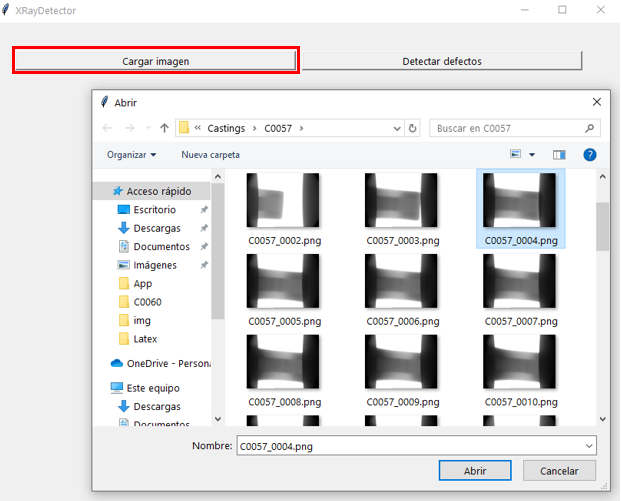
\includegraphics[scale=0.8]{carga_imagen}
	\caption{Carga de una imagen en la aplicación}
	\label{carga_imagen}
\end{figure}

\subsection{Detectar defectos}

Para detectar los defectos de la imagen cargada:

\begin{enumerate}
    \item Hacer click en el botón ``Detectar defectos''.
    \item Espere, el proceso puede tardar unos segundos.
    \item La imagen con los defectos aparecerá en la aplicación.
\end{enumerate}

\imagen{detectar_defectos}{Detectar defectos de una imagen\label{detectar_defectos}}

\newpage

\subsection{Visualizar máscaras}

Para visualizar las máscaras de la imagen:

\begin{enumerate}
    \item Hacer click en el botón ``Máscaras''.
    \item Se abre una segunda ventana con la/s imágenes de las máscaras.
\end{enumerate}

\begin{figure}[H]
	\centering
	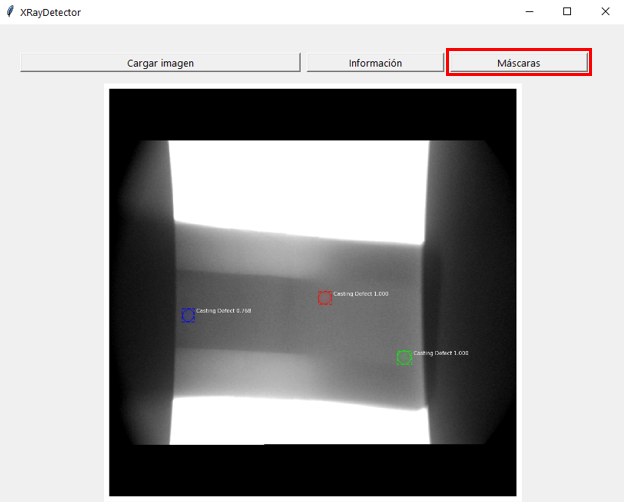
\includegraphics[scale=0.7]{visualizar_mascaras}
	\caption{Visualizar las máscaras de los defectos de la imagen}
	\label{visualizar_mascaras}
\end{figure}

\imagen{mascara_cargada}{Máscaras de los defectos de la imagen\label{mascara_cargada}}

\subsection{Información de los defectos}

Para ver la información sobre los defectos detectados en la imagen:

\begin{enumerate}
    \item Hacer click en el botón ``Información''.
    \item Se abre una segunda ventana con la información de los defectos.
\end{enumerate}

\imagen{informacion_defectos}{Visualizar la información de los defectos de la imagen\label{informacion_defectos}}

\begin{figure}[htb]
	\centering
	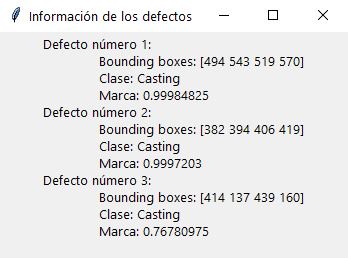
\includegraphics[width=0.53\textwidth]{informacion_cargada}
	\caption{Información de los defectos de la imagen}
	\label{informacion_cargada}
\end{figure}

\newpage

\subsection{Errores}

Los errores controlados que pueden salir son:

\begin{enumerate}
    \item Se produce algún problema al cargar la imagen, mensaje: ``Error al cargar la imagen.''. Ver figura \ref{error_carga}.
    \item Se carga un archivo que no es una imagen, mensaje: ``El archivo no es una imagen.''. Ver figura \ref{archivo_no_imagen}.
    \item Se selecciona un directorio que no existe, mensaje: ``El directorio no existe.''. Ver figura \ref{no_existe_directorio}.
    \item Se hace click en el botón ``Detectar defectos'' sin haber cagado la imagen, mensaje: ``No hay una imagen cargada.''. Ver figura \ref{no_imagen_cargada}.
    \item Se produce algún problema al cargar la imagen después de detectar los defectos, mensaje: ``Error al cargar la imagen.''. Ver figura \ref{error_carga}.
    \item No haya defectos en la imagen y se hace click en el botón ``Máscaras'', mensaje: ``No hay defectos en la imagen.''. Ver figura \ref{no_defectos}.
    \item No haya defectos en la imagen y se hace click en el botón ``Información'', mensaje: ``No hay defectos en la imagen.''. Ver figura \ref{no_defectos}.
\end{enumerate}

\begin{figure}[htb]
	\centering
	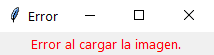
\includegraphics[width=0.7\textwidth]{error_carga}
	\caption{Problema al cargar la imagen}
	\label{error_carga}
\end{figure}

\begin{figure}[htb]
	\centering
	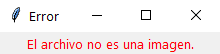
\includegraphics[width=0.7\textwidth]{archivo_no_imagen}
	\caption{El archivo cargado no es una imagen}
	\label{archivo_no_imagen}
\end{figure}

\begin{figure}[htb]
	\centering
	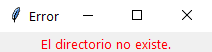
\includegraphics[width=0.7\textwidth]{no_existe_directorio}
	\caption{No existe el directorio seleccionado}
	\label{no_existe_directorio}
\end{figure}

\begin{figure}[htb]
	\centering
	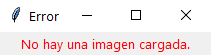
\includegraphics[width=0.7\textwidth]{no_imagen_cargada}
	\caption{No hay una imagen cargada para detectar defectos}
	\label{no_imagen_cargada}
\end{figure}

\begin{figure}[htb]
	\centering
	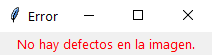
\includegraphics[width=0.7\textwidth]{no_defectos}
	\caption{No hay defectos detectados en la imagen}
	\label{no_defectos}
\end{figure}